\documentclass{scrartcl}

\usepackage{amssymb}
\usepackage{amsmath}
\usepackage{tikz}
\usetikzlibrary{patterns}

%from Althusser - Philosophy and the Spontaneous Philosophy of the Scientists

%N1 = Nucleus 1
%N2 = Nucleus 2
%SPS = Spontaneous Philosophy of the Scientist
%WV = World-View
%S = Science
%\Phi = Philosophy

\begin{document}
	
	\begin{figure}
		\centering
		%\hspace{1.25cm}
	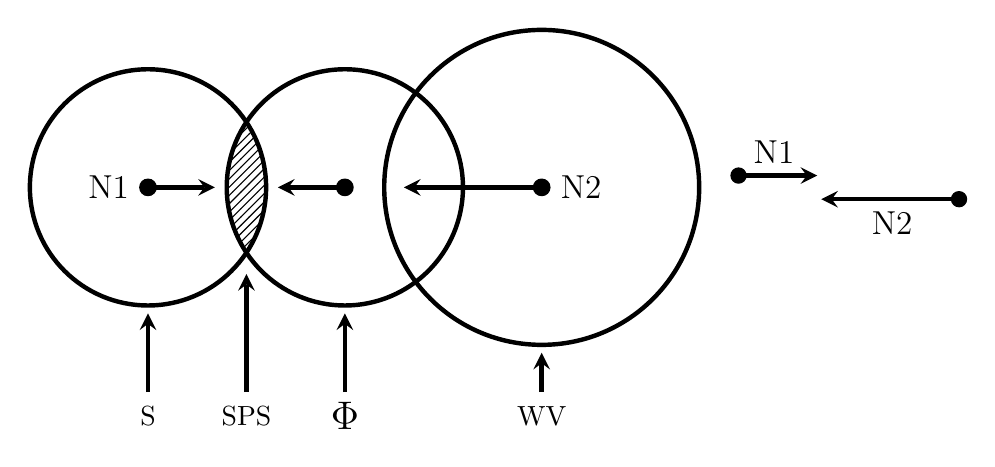
\begin{tikzpicture}[>=stealth]
	%circles
	\draw[ultra thick] (0,0) circle (2cm);
	\draw[ultra thick] (-2.5,0) circle (1.5cm);
	\draw[ultra thick] (-5,0) circle (1.5cm);
	
	%black dots
	\node[circle,draw=black, fill=black, inner sep=0pt,minimum size=6pt] at (0,0) {};
	\node[circle,draw=black, fill=black, inner sep=0pt,minimum size=6pt] at (-2.5,0) {};
	\node[circle,draw=black, fill=black, inner sep=0pt,minimum size=6pt] at (-5,0) {};
	%
	\node[circle,draw=black, fill=black, inner sep=0pt,minimum size=5.5pt] at (2.5,0.15) {};
	\node[circle,draw=black, fill=black, inner sep=0pt,minimum size=5.5pt] at (5.3,-0.15) {};
	
	%horizontal arrows
	\draw[->,ultra thick] (0,0)--(-1.75,0);				%rightmost
	\draw[->,ultra thick] (-2.5,0)--(-3.35,0);			%center
	\draw[->,ultra thick] (-5,0)--(-4.15,0);			%leftmost
	%
	\draw[->,ultra thick] (2.5,0.15)--(3.5,0.15);		%N1
	\draw[->,ultra thick] (5.3,-0.15)--(3.55,-0.15);	%N2
	
	%vertical arrows
	\draw[->,ultra thick] (0,-2.6)--(0,-2.1);			%WV
	\draw[->,ultra thick] (-2.5,-2.6)--(-2.5,-1.6);		%\Phi
	\draw[->,ultra thick] (-3.75,-2.6)--(-3.75,-1.1);	%SPS
	\draw[->,ultra thick] (-5,-2.6)--(-5,-1.6);			%S
	
	%labels
	\node at (-5.5,0) {{\large N1}};
	\node at (0.5,0)  {{\large N2}};
	%
	\node at (2.95,0.45)  {{\large N1}};
	\node at (4.45,-0.45) {{\large N2}};
	%
	\node at (0,-2.9)    {WV};
	\node at (-2.5,-2.9) {{\Large $\Phi$}};
	\node at (-3.75,-2.9){SPS};
	\node at (-5,-2.9)   {S};
	
	%hatched intersection
	\clip (-2.5,0) circle (1.5cm); 			%keep only what is inside center circle
	\draw[pattern=north east lines, pattern color=black] (-5,0) circle (1.5cm);  %draw left circle
	%code via: http://users.ju.edu/hduong/math220/venn_diagrams.pdf
	\end{tikzpicture}
		\caption{Representing the existence of \textit{two irradiating nuclei}}
		\vspace*{5in}	%this is just for spacing; otherwise, it goes to middle of page
	\end{figure}
	
\end{document}